\documentclass[10pt]{article}
\usepackage[utf8]{inputenc}
\usepackage[T1]{fontenc}
\usepackage{amsmath}
\usepackage{amsfonts}
\usepackage{amssymb}
\usepackage[version=4]{mhchem}
\usepackage{stmaryrd}
\usepackage{graphicx}
\usepackage[export]{adjustbox}
\graphicspath{ {./images/} }
\usepackage{caption}

%New command to display footnote whose markers will always be hidden
\let\svthefootnote\thefootnote
\newcommand\blfootnotetext[1]{%
  \let\thefootnote\relax\footnote{#1}%
  \addtocounter{footnote}{-1}%
  \let\thefootnote\svthefootnote%
}

%Overriding the \footnotetext command to hide the marker if its value is `0`
\let\svfootnotetext\footnotetext
\renewcommand\footnotetext[2][?]{%
  \if\relax#1\relax%
    \ifnum\value{footnote}=0\blfootnotetext{#2}\else\svfootnotetext{#2}\fi%
  \else%
    \if?#1\ifnum\value{footnote}=0\blfootnotetext{#2}\else\svfootnotetext{#2}\fi%
    \else\svfootnotetext[#1]{#2}\fi%
  \fi
}

\begin{document}

\section*{13 Relativistic Beaming (50 Points)}
Consider an isotropic light source of frequency $f_{R}$ in a frame which is fixed to the source (i.e. rest frame). In this rest frame, consider a light ray emitted from the source that makes an angle $\theta_{R}$ with the $X$-axis. The light source is moving along positive $X$ direction with (relativistic) speed $v$ as measured in the lab frame.\\
(a) Find an expression for the frequency $f_{L}$ of this ray in the lab frame, and the cosine of the angle that this ray makes with the $X$-axis in the lab frame.

Hint: In relativistic mechanics, energy $E$ and momentum $p$ of a particle between rest and lab frame are related in the following way:

$$
\begin{aligned}
\frac{E_{L}}{c} & =\gamma\left(\frac{E_{R}}{c}+p_{x_{R}} \frac{v}{c}\right) \\
p_{x_{L}} & =\gamma\left(p_{x_{R}}+\frac{E_{R} v}{c^{2}}\right) \\
p_{y_{L}} & =p_{y_{R}} \\
p_{z_{L}} & =p_{z_{R}}
\end{aligned}
$$

where:

$$
\gamma=\frac{1}{\sqrt{1-\frac{v^{2}}{c^{2}}}}
$$

(b) For the following cases:\\
i) $\theta_{R}=0^{\circ}$\\
ii) $\theta_{R}=\cos ^{-1}(-v / c)$\\
iii) $\theta_{R}=90^{\circ}$\\
iv) $\theta_{L}=180^{\circ}$\\
draw direction vectors of the beam in $X Y$ plane of the rest frame as well as separately in $X^{\prime} Y^{\prime}$ plane of the lab frame.

In accretion disks around black holes, the charged particles are orbiting at relativistic speeds and in their rest frames may be considered as isotropic point sources of light. Consider such a particle $K$ in a circular orbit of radius $r$ and angular speed $\omega$ around a central object located at $O$ (see figure).\\
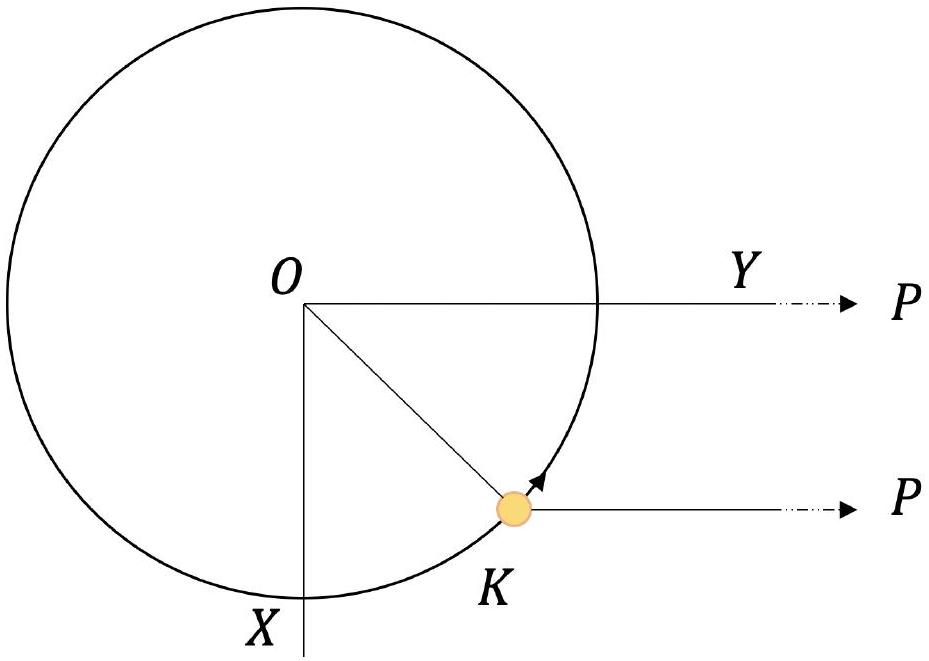
\includegraphics[max width=\textwidth, center]{2025_09_11_6312450c103d6a7e5736g-10}

Let us assume that our lab frame is fixed to an observer located at a point $P$ on the $O Y$ axis, which is stationary with respect to $O . O P=R \gg r$. Let $t_{L 0}=t_{R 0}=0$ correspond to the moment when K is seen crossing the OX axis. As $K$ is moving with relativistic speed, the duration $\Delta t_{R}$ measured by an observer in the rest frame of the source $K$ is related to the duration measured in the lab frame $\Delta t_{L}$ at $P$ by the expression $\Delta t_{L}=\gamma \Delta t_{R}$.\\
(c) Derive an expression for $f_{L}$ as a function of $t_{L}\left(t_{L}>R / c\right)$ ?

Let us consider a fraction of the light from the source that is emitted in an infinitesimal solid angle $\Delta \Omega_{R}=-\Delta\left(\cos \theta_{R}\right) \cdot \Delta \phi$ in the direction making an angle $\theta_{R}$ with respect to the $X$ axis in the rest frame, as it is shown on the figure below.\\
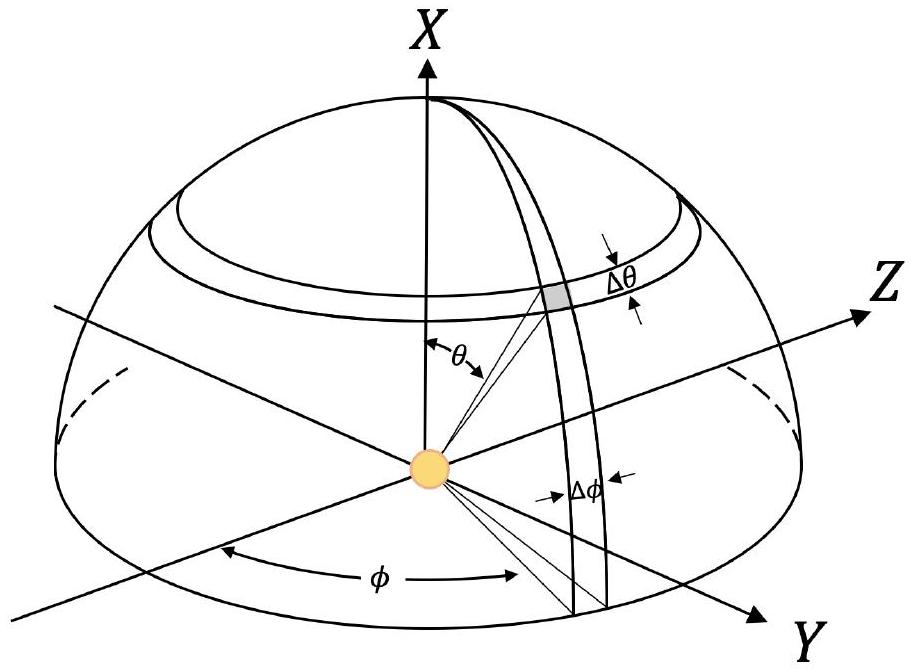
\includegraphics[max width=\textwidth, center]{2025_09_11_6312450c103d6a7e5736g-10(1)}\\
(d) Show that, as measured in the lab frame


\begin{equation*}
\Delta \Omega_{L}=\frac{\Delta \Omega_{R}}{\gamma^{2}\left(1+\frac{v}{c} \cos \theta_{R}\right)^{2}} \tag{10pt}
\end{equation*}


(e) If the intrinsic luminosity of the light source is $L$, what is the energy flux $F_{L}$ observed by the observer at point $P$ at the moment $t_{L}\left(t_{L}>R / c\right)$ ?

Hint: In the rest frame of the source, you may assume $N_{R}$ number of photons are directed within the solid angle $\Delta \Omega_{R}$ during the time interval $\Delta t_{R}$.\\
(f) Charged particles in the relativistic beam shot from the supermassive black hole at the centre of the galaxy M87 have speeds up to 0.95 c . What would be the maximum and minimum amplification factor for the energy flux for a relativistic beam from M87?

\end{document}